% !TEX root = main.tex
\section{Experiments}
\subsection{Dataset}
Our dataset consists of 30 high level natural language instructions taken using a \href{http://52.25.65.189:9000/#/getFeedback}{crowd sourcing system}. The instructions are taken for 16 different environments depicting scenes similar to living room, bedroom and kitchen. \\
The environments are constructed in OpenRAVE with context generating from 6 different human activities depicted by skeletals. The activities considered are walking, watching, interacting, reaching, sitting and working. \\
The instructions involve task description for themes in common house-hold enviromnent like cleaning the room, arranging the guest room and serving coffee. The dataset contains considerable high level instructions like distribute, arrange etc. with variety in verbs.\\
We filtered out 2 datapoints containing instructions which were very high level and uncertain even for  humans. Of the 30 valid datapoints, 16 are used for training and 14 are used for testing purposes.  

Please see supplementary for examples from our dataset.

\subsection{Set Up:}
	\subsubsection{Planit with Coactive Feedback:} 
		Training Set : 7 different environments with different activities occuring in them. User was shown trajectories for going from one point to another and the user can stop trajectories and update specific waypoints of the trajectory by dragging the waypoint to a better point. Total 432 feedback was collected from the user. For evaluation, considered a set of 10 environments, 7 existing+3 new. The parameters were used to rank 112 trajectory sets each containing 7 trajectories. Original version of planit ( as reported in the planit paper (expert system) was assumed as the ground truth. \textbf{The nDCG for the above system was 0.782727868206}. This is reasonable since in the earlier version the feedback was expert (labelling segments of 2500 different trajectories) and in the given system we have just 400 feedback.\ref{fig:planitResult} 
		% 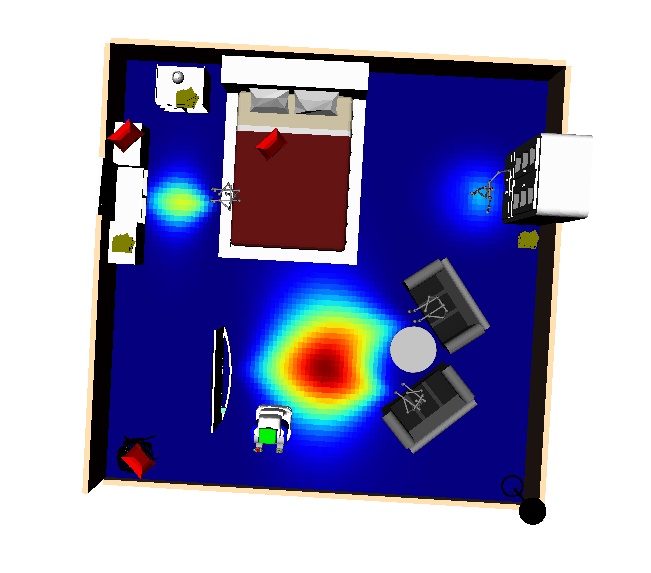
\includegraphics[scale=0.5]{planitResult}
		\begin{figure}[h]
		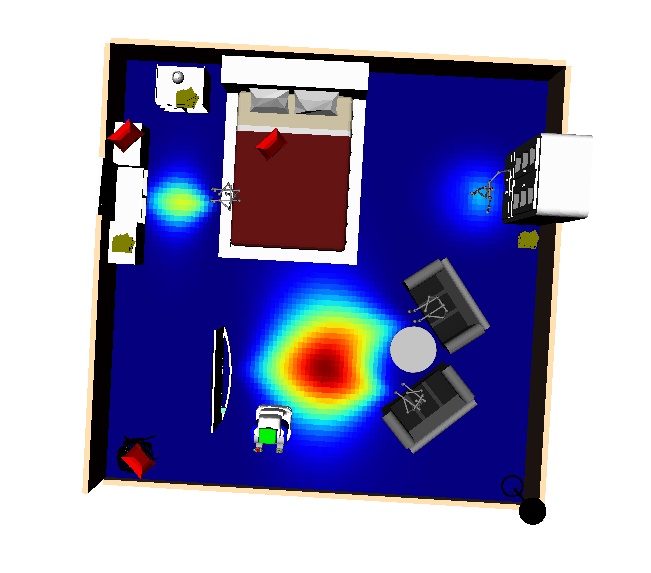
\includegraphics[width=5cm]{planitResult}
		\centering
		\caption{Cost function learnt via Coactive Feedback}
  		\label{fig:planitResult}
		\end{figure}


\subsection{Results} \todo{Dip: please take a detailed pass over this subsection}
We test our algorithm on two tasks, in the first task we evaluate the success of co-active feedback in tuning the robot system and in second task, we evaluate the results from different type of feedback.

\noindent\textit{Task 1: Improvement Due to Co-active feedback}
\textit{Conclusion:} The system is able to improve its accuracy by BLAH on a held-out test set, after a few iterations of co-active feebacks from non-expert users.

\begin{table}
\label{tbl:tsk1}
\caption{Table 1: System improves its end-to-end accuracy after receiving co-active feedback on the final robot behavior}
\centering
\begin{tabular}{|l|l|}
\hline
\textit{System} & \textit{Accuracy} \\
\hline
Sys & BLAH \\
Sys + CF & BLAH \\
Sys + MCF & BLAH \\
\hline
\end{tabular}
\end{table}

\noindent\textit{Task 2: Effects of Different Type of Feedback}
\textit{Conclusion:} Our system based on co-active feedback is able to achieve close performance with system using expert feedback. Further, our system vastly outperforms system based on boolean feedback.

\begin{table}
\label{tbl:tsk2}
\caption{Table 2: Co-active feedback achieves close to the performance with expert feedback}
\centering
\begin{tabular}{|l|l|}
\hline
\textit{System} & \textit{Accuracy} \\
\hline
Sys + boolean & BLAH\\
Sys + CF & BLAH \\
Sys + Expert & BLAH \\
\hline
\end{tabular}
\end{table}


\todo{Dip: we should also experiment with individually tuning the two system AND experiment with different number of feedback until an asymptote is attained}
